\documentclass[12pt]{book}
\usepackage{graphicx}
\title{Resultaten}
\author{J.F.J. Blom}
\date{\today}
\begin{document}
\section*{Resultaten en Discussie}
Er zijn vier verschillende metingen verricht, kalibratiemeting, onbekende afstandsmeting en de lineariteitsmeting. In dit hoofstuk zijn alle meetresultaten weergeven en geanalyseerd.Van alle meetresultaten is het gemiddelde genomen, doormiddel van deze formule:
$$\frac{\sum_{i=1}^{n}x_i}{n}$$
Hier is $x_i$ een meetresultaat en n is het aantal metingen. 
Daarnaast is de onzekerheid van de metingen berekend. Daarbij is gebruik gemaakt van de volgende formule:
$$\sqrt{\frac{\sum_{i=1}^{n}( x_i-x_a)^2}{n(n-1)}}$$
$x_a$ is hier het gemiddelde van de meting.
\subsection*{Kalibratie}
Hieronder zijn de meetresultaten van de kalibratiemeting te zien. De meetresultaten zijn vrij constant, en dus is de onzekerheid vrij laag. De onzekerheid van de tijdsmeting is vastgesteld op 0.003 seconden, waaruit blijkt dat de meting erg accuraat is. De onzekerheid van de snelheid wordt dan 0.025 cm/s. 

\begin{center}
\begin{tabular}{| l| c|}
\hline
    & Kalibratie 10 cm \\
\hline
   Meting 1 (s) & 1.031 \\
\hline
   Meting 2 (s) & 1.042 \\
\hline
   Meting 3 (s) & 1.042 \\
\hline
   Meting 4 (s) & 1.046 \\
\hline
   Meting 5 (s) & 1.045 \\
\hline
   Gemiddelde (s) & 1.041 \\
\hline
   Gemiddelde snelheid (cm/s) & 9.602 \\
\hline
   Onzekerheid tijd (s) & 0.003 \\
\hline
   Onzekerheid snelheid (cm/s) & 0.025 \\
\hline
\end{tabular}
\end{center}

\subsection*{Onbekende afstand}
Hieronder zijn de meetresultaten te zien van de onbekende afstandsmeting. Om de snelheid te kunnen bepalen moet er een afstand bekend zijn. Deze afstand is gemeten en deze is 23.4 cm. De onzekerheid van de tijdsmeting is vastgesteld op 0.005 seconden, en dus is de meting erg nauwkeurig. Deze meting is zoals verwacht vanwege de langere afstand iets minder accuraat als de kalibratiemeting. De onzekerheid van de snelheid is vastgesteld op 0.007 cm/s, en dus is ook deze meting erg nauwkeurig.
\begin{center}
\begin{tabular}{| l| c|}
\hline
    & Onbekende afstand 23.4 cm\\
\hline
   Meting 1 (s) & 2.526 \\
\hline
   Meting 2 (s) & 2.531 \\
\hline
   Meting 3 (s) & 2.515 \\
\hline
   Meting 4 (s) & 2.518 \\
\hline
   Meting 5 (s) & 2.522 \\
\hline
   Gemiddelde (s) & 2.523 \\
\hline
   Gemiddelde snelheid (cm/s) & 9.276 \\
\hline
   Onzekerheid tijd (s) & 0.005 \\
\hline
   Onzekerheid snelheid (cm/s) & 0.007 \\
\hline
 \end{tabular}
\end{center}

\subsection*{Lineariteit}
Hieronder zijn de meetresultaten te zien van de lineariteitsmeting. Om de zien hoe lineair de afstandsmeter van de robot is, moet de  onzekerheid van de gemiddelde snelheden uitgerekent worden
\begin{center}
\begin{tabular}{| l| c| c| c| c| c|}
\hline
   & 5 cm & 10 cm & 15 cm & 20 cm & 25 cm\\
\hline
   Meting 1 (s) & 0.542 & 1.092 & 1.638 & 2.218 & 2.728 \\
\hline
   Meting 2 (s) & 0.550 & 1.086 & 1.636 & 2.237 & 2.747 \\
\hline
   Meting 3 (s) & 0.547 & 1.089 & 1.627 & 2.210 & 2.728 \\
\hline
   Meting 4 (s) & 0.548 & 1.081 & 1.634 & 2.218 & 2.724 \\
\hline
   Meting 5 (s) & 0.542 & 1.081 & 1.658 & 2.233 & 2.733 \\
\hline
   Gemiddelde (s) & 0.546 & 1.086 & 1.638 & 2.223 & 2.732 \\
\hline
   Gemiddelde snelheid (cm/s) & 9.164 & 9.211 & 9.155 & 8.996 & 9.151 \\
\hline
   Onzekerheid tijd (s) & 0.002 & 0.002 & 0.005 & 0.005 & 0.004 \\
\hline
   Onzekerheid snelheid (cm/s) & 0.055 & 0.018 & 0.019 & 0.10 & 0.005 \\
\hline
 \end{tabular}
\end{center}
\begin{center}
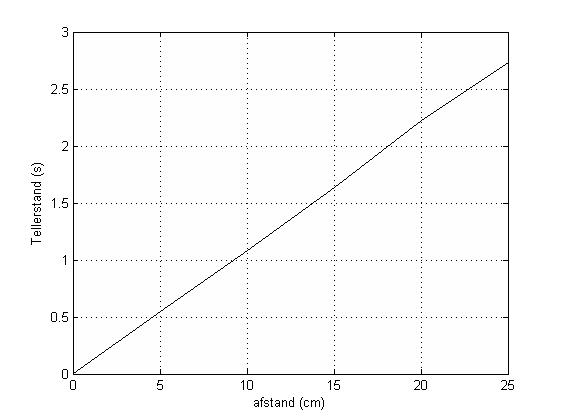
\includegraphics[width=150mm] {afstand-tellerstand.jpg}
\end{center}
In de bovenstaande grafiek is de afstand afgezet tegen de tellerstand van de robot. De lijn is bijna recht, dus de afstandsmeter van de robot is ook bijna lineair. Op de volgende pagina zet ik de afstand af tegen de snelheid, waardoor de afwijkingen in lineariteit beter te zien zijn. 
\begin{center}
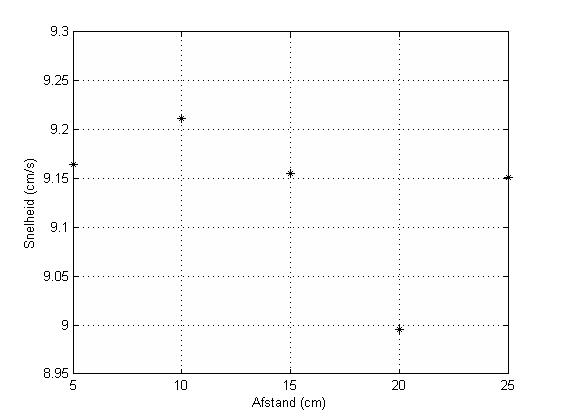
\includegraphics[width=150mm] {afstand-snelheid.jpg}
\end{center}
In de bovenstaande grafiek is de afstand afgezet tegen de ssnelheid. Hier zijn goed de afwijkingen in lineariteit van de afstandsmeter te zien. De snelheid blijft tussen de 9.22 en de 8.99 en de snelheid is dus vrij constant. De afstandsmeter is dus bohoorlijk lineair. 
\section*{Conclusie}

\end{document}